\documentclass[oneside,final,14pt,a4paper]{extreport}

\usepackage{tempora}   

\usepackage{vmargin}
\setpapersize{A4}
\setmarginsrb{2.5cm}{2.2cm}{2.2cm}{2.2cm}{0pt}{10mm}{0pt}{13mm}
\usepackage{setspace}
\sloppy
\setstretch{1.5}
\usepackage{indentfirst}
\parindent=1.25cm

%%%%% ADDED TO SUPPORT TT BOLD FACES %%%%
\DeclareFontShape{OT1}{cmtt}{bx}{n}{<5><6><7><8><9><10><10.95><12><14.4><17.28><20.74><24.88>cmttb10}{}
\renewcommand{\ttdefault}{pcr}
%%%%% END %%%%%%%%%%%%%%%%%%%%%%%%%%%%%%% 
\usepackage{atbegshi,picture}
\usepackage[T1,T2A]{fontenc} 
\usepackage[utf8]{inputenc}
\usepackage[main=russian,english]{babel}
\usepackage[backend=biber,style=ieee,autocite=inline]{biblatex}
\bibliography{ref.bib}
\usepackage{csquotes}
\usepackage{blindtext}


\usepackage{pdfpages}
\newenvironment{bottompar}{\par\vspace*{\fill}}{\clearpage}

% \usepackage{cite}
\usepackage{amsmath,amsfonts}
\usepackage{amsthm}
\newtheorem{theorem}{Theorem}
\newtheorem{corollary}{Corollary}
\newtheorem{lemma}{Lemma}
\newtheorem{proposition}{Proposition}
\theoremstyle{definition}
\newtheorem{definition}{Definition}
\theoremstyle{remark}
\newtheorem*{remark}{Remark}
\theoremstyle{remark}
\newtheorem*{example}{Example}



\usepackage{graphicx}
\graphicspath{{figs/}} %path to images
\usepackage{multirow,array}
\usepackage{caption}
\usepackage{subcaption}
\usepackage[unicode]{hyperref}
\hypersetup{colorlinks=true, linkcolor=black, citecolor=black}
\usepackage{paralist}
\usepackage{listings}
\usepackage{zed-csp}
\usepackage{fancyhdr}
\usepackage{color,colortbl}
\usepackage{booktabs}
\usepackage{epsfig} % for postscript graphics files

\usepackage{upgreek} 
\usepackage{bm}
\usepackage{hyperref}
\usepackage{longtable}
\usepackage[font=singlespacing, labelfont=bf]{caption}
\usepackage{floatrow}

\usepackage{etoolbox}

\makeatletter
% \chapter без перехода на новую страницу
\patchcmd{\chapter}{\clearpage}{\par}{}{}
\patchcmd{\chapter}{\cleardoublepage}{\par}{}{}
\patchcmd{\chapter}{\thispagestyle{plain}}{}{}{}
% Уменьшаем верхний отступ заголовка главы
\patchcmd{\@makechapterhead}{\vspace*{50\p@}}{\vspace*{20\p@}}{}{}
\patchcmd{\@makeschapterhead}{\vspace*{50\p@}}{\vspace*{20\p@}}{}{}
\makeatother

\usepackage{titlesec}

% Делаем \chapter заголовком в потоке текста, без разрыва страницы
\titleformat{\chapter}[hang]
  {\normalfont\Large\bfseries}   % шрифт заголовка
  {\thechapter}                   % номер
  {1em}                           % отступ между номером и текстом
  {}                              % код перед текстом
\titlespacing*{\chapter}
  {0pt}        % левый отступ
  {3.5ex plus 1ex minus .2ex}     % отступ сверху
  {2.3ex plus .2ex}      


\pagestyle{fancyplain}

% remember section title
\renewcommand{\chaptermark}[1]%
	{\markboth{\chaptername~\thechapter~--~#1}{}}

% subsection number and title
\renewcommand{\sectionmark}[1]%
	{\markright{\thesection\ #1}}

\rhead[\fancyplain{}{\bf\leftmark}]%
      {\fancyplain{}{\bf\thepage}}
\lhead[\fancyplain{}{\bf\thepage}]%
      {\fancyplain{}{\bf\rightmark}}
\cfoot{} %bfseries


\newcommand{\dedication}[1]
   {\thispagestyle{empty}
     
   \begin{flushleft}\raggedleft #1\end{flushleft}
}

\begin{document}

\fancypagestyle{plain}{%
  \fancyhf{}%
  \fancyhead[R]{\bfseries\thepage}%
  \renewcommand{\headrulewidth}{0pt}%
}

% Титул
\pagestyle{empty}
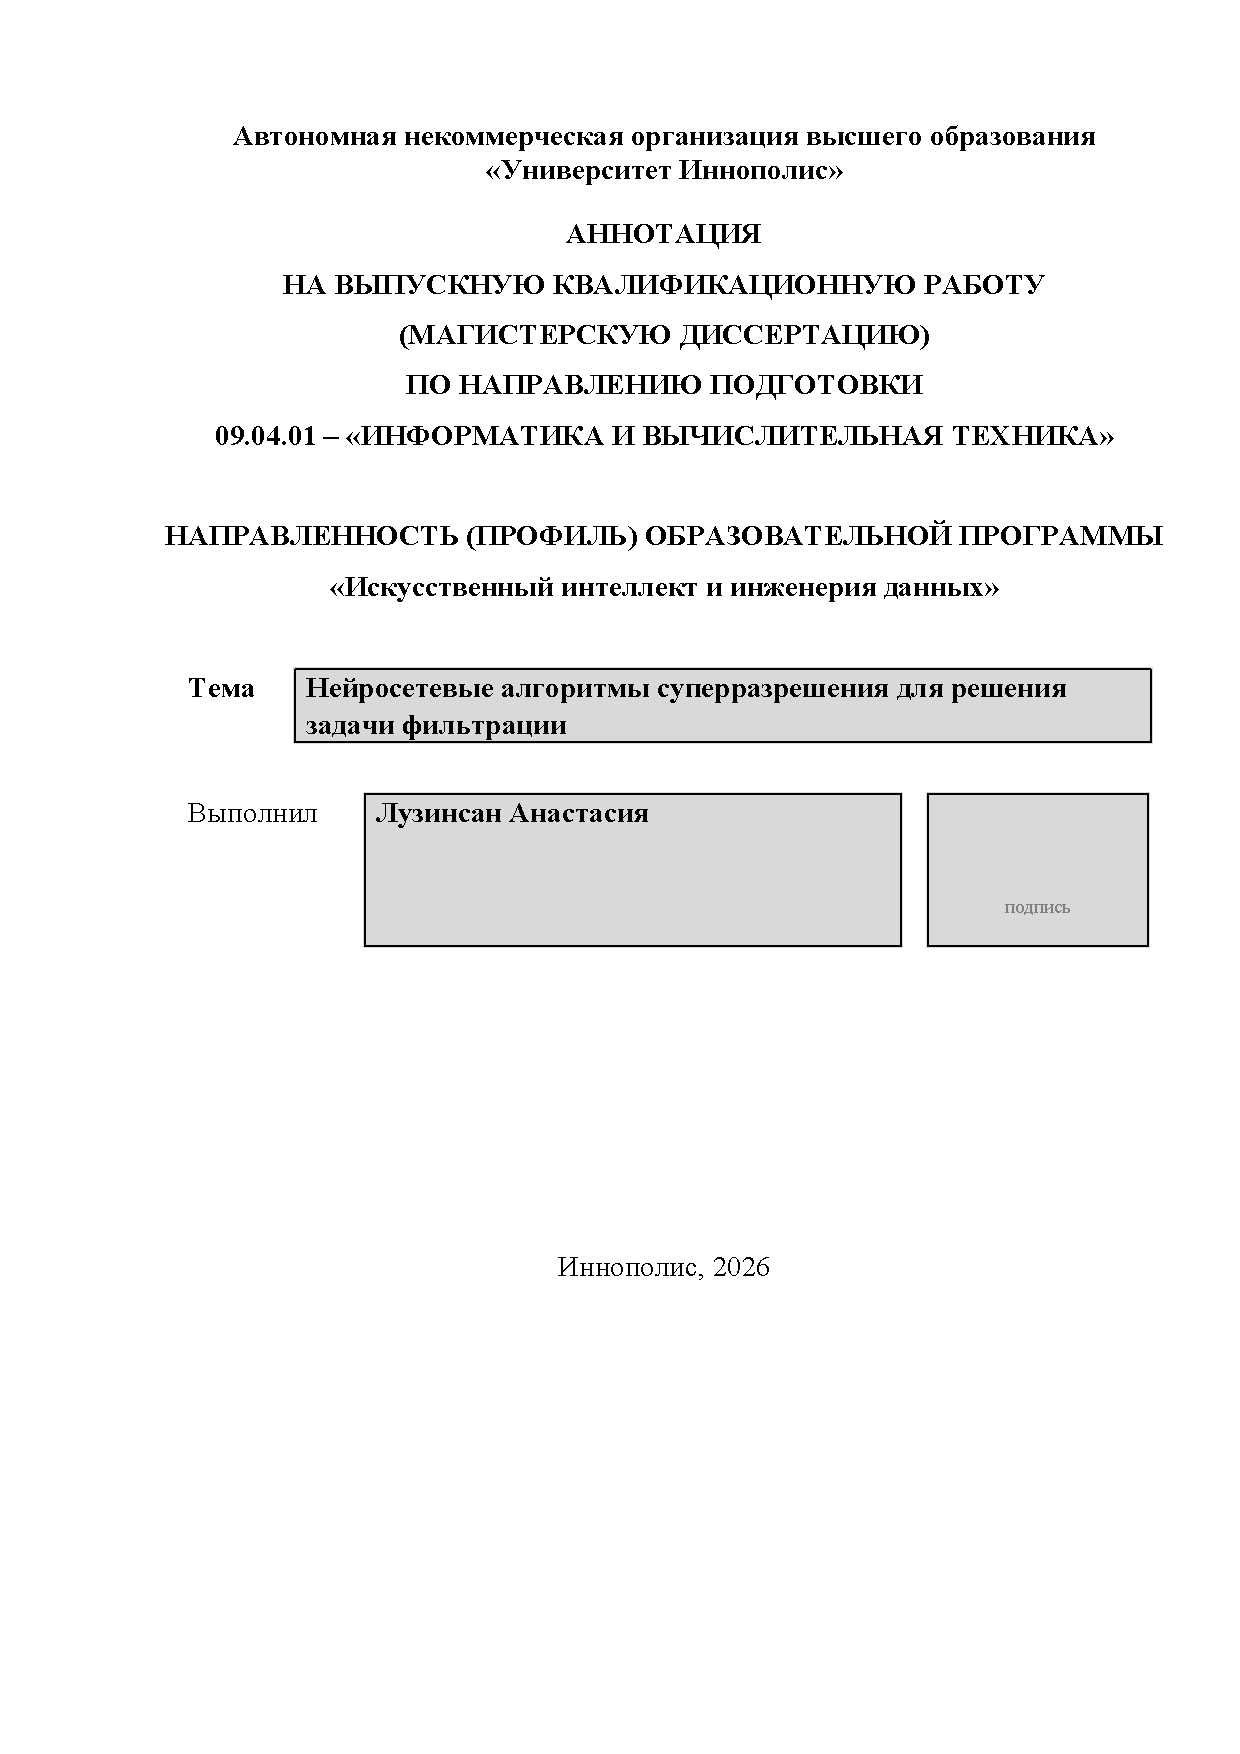
\includepdf[pages=-, offset=70 -70]{Annotation.pdf}

% Содержание
\newpage
\tableofcontents
\thispagestyle{empty}
\newpage

% Основная часть
\pagestyle{fancyplain}
\setcounter{page}{3}

\chapter{Введение}
\label{chap:intro}

При гидродинамическом моделировании нефтяных пластов приходится искать компромисс между точностью и вычислительными затратами: детальная сетка отслеживает фронты вытеснения, но требует больших ресурсов, а укрупнение сетки ускоряет расчет ценой размытия фронта и завышения прогноза нефтедобычи. Классические методы интерполяции здесь бессильны: работая как фильтры нижних частот, они сглаживают картинку, не восстанавливая утраченные высокочастотные детали.

Цель работы — создать программный комплекс на базе нейросетевых подходов для быстрого и точного восстановления нестационарных полей давления и насыщенности по расчетам на грубой сетке. Подход использует суперразрешение на сверточных сетях, обученных на парах согласованных данных: быстрых расчетах на грубой сетке и эталонных — на детальной, полученных моделью трещиновато-пористых коллекторов.
\chapter{Обзор литературы}
\label{chap:lr}

Многофазная фильтрация в трещиновато-пористых пластах описывается связанной системой нелинейных уравнений для трёх полей: давления, водонасыщенности трещин и матричных блоков. Её решения содержат подвижные резкие фронты вытеснения, которые грубые разностные схемы аппроксимируют неудовлетворительно, а уменьшение шага сетки выводит полномасштабную модель в область неприемлемых вычислительных затрат.

Постановка восстановления детальных полей по грубым приближениям совпадает с задачей сверхразрешения изображений. Сверточные и остаточные архитектуры точны по среднеквадратичной метрике, но сглаживают высокочастотное содержание~\autocite{lim2017enhanced}; состязательное обучение (GAN) восстанавливает резкие границы~\autocite{cvf_srgan}. В нефтяной инженерии суперразрешение уже применялось к полям насыщенности и течения, в том числе с физически обоснованной регуляризацией~\autocite{li2025spe}.

Ключевое ограничение опубликованных работ — применимость только к однопоровым моделям. Задача одновременного восстановления трёх связанных полей для систем двойной пористости в литературе до настоящего времени не рассматривалась, что определяет научную новизну работы.
\chapter{Методология}
\label{chap:methodology}


\chapter{Результаты}
\label{chap:results}

В таблице~\ref{tab:val_metrics} приведены валидационные метрики шести моделей относительно порогов приёмки. После регрессионной стадии порог по PSNR проходят два глубоких генератора, а по SSIM не проходит ни один. После состязательного дообучения все три модели укладываются во все пороги, причём PSNR и SSIM растут одновременно. Наилучшие значения по всем метрикам показывает RFDN GAN, остающийся при этом самым компактным: около 3 МБ в формате ONNX против 5.8 МБ у EDSR.

\begin{table}[h]
\captionsetup{justification=centering}
\centering
\caption{Валидационные метрики относительно порогов приёмки.}
\label{tab:val_metrics}
\small
\setlength{\tabcolsep}{6pt}
\begin{tabular}{l cccc}
\toprule
Конфигурация
  & PSNR$\uparrow$ & SSIM$\uparrow$ & GMAE$\downarrow$ & ERGAS$\downarrow$ \\
Порог
  & $\geq 45$ & $\geq 0.55$ & $\leq 0.002$ & $\leq 0.4$ \\
\midrule
\multicolumn{5}{l}{Регрессионная стадия} \\
\midrule
MSRResNet & 44.92          & \textbf{0.559} & \textbf{0.00195} & \textbf{0.380} \\
EDSR      & \textbf{46.92} & 0.548          & \textbf{0.00064} & \textbf{0.272} \\
RFDN      & \textbf{46.11} & 0.505          & \textbf{0.00083} & \textbf{0.310} \\
\midrule
\multicolumn{5}{l}{Состязательное дообучение} \\
\midrule
MSRResNet GAN & \textbf{45.99} & \textbf{0.590} & \textbf{0.00165} & \textbf{0.353} \\
EDSR GAN      & \textbf{47.71} & \textbf{0.606} & \textbf{0.00062} & \textbf{0.257} \\
RFDN GAN      & \textbf{47.77} & \textbf{0.634} & \textbf{0.00070} & \textbf{0.264} \\
\bottomrule
\end{tabular}
\end{table}
\chapter{Выводы}
\label{chap:conclusion}

Гипотеза о влиянии глубины подтвердилась лишь частично: ёмкость сети управляет поэлементной точностью, но структурное качество от неё почти не зависит и при чисто пиксельном обучении остаётся ниже приемлемого. Гипотеза о состязательном дообучении верна без оговорок, причём свойственный классическим SR-GAN компромисс между точностью и резкостью здесь не возникает: добавление физического регуляризатора удерживает обе группы метрик. Отсюда главный практический вывод: самая компактная модель не уступает тяжёлым, а по структуре даже превосходит их.

Достигнутый уровень структурного качества, по-видимому, упирается в небольшой обучающий набор, поэтому первоочередным направлением дальнейшей работы остаётся его расширение и пополнение более разнообразными режимами фильтрации.

\printbibliography[heading=bibintoc,title={Список использованной литературы}]

\end{document}
